\documentclass[10pt]{amsart} % use larger type; default would be 10pt
\usepackage{color}
\usepackage[utf8]{inputenc} % set input encoding (not needed with XeLaTeX)



%%% PACKAGES
\usepackage{booktabs}
\usepackage{array} 

\usepackage{amsfonts}
\usepackage{amsthm}
\usepackage{tikz}
\usepackage{amsmath}
\usepackage{float}
\usepackage{graphicx}
\usepackage{caption}
\usepackage{subcaption}
\usepackage{color}

\newtheorem{theorem}{Theorem} 
\newtheorem{lemma}{Lemma}
\newtheorem{propn}{Proposition}
\newtheorem*{thmm}{Theorem}
\newtheorem{remk}{Remark} 
\newtheorem{corol}{Corollary}
\newtheorem{definition}{Definition}



\newtheorem{thm}{Theorem}[section] 
\newtheorem{prop}[thm]{Proposition} 
\newtheorem{lem}[thm]{Lemma}
\newtheorem{cor}[thm]{Corollary} 
\newtheorem{con}[thm]{Conjecture} 

\theoremstyle{definition}
\newtheorem{defn}[thm]{Definition}
\newtheorem*{rem}{Remark}
\newtheorem*{nota}{Notation}
\newtheorem{cla}[thm]{Claim}
\newtheorem{ex}[thm]{Example}
\newtheorem{exs}[thm]{Examples}
\newtheorem*{exer}{Exercise}
\newtheorem{case}{Case}

\definecolor{sotonblue}{rgb}{0.0,0.394,0.597}
\title{Some probabilities}
\author{David Matthews}
\DeclareMathOperator{\vol}{vol}
\DeclareMathOperator{\Vol}{Vol}
\DeclareMathOperator{\Sym}{Sym}
\DeclareMathOperator{\lv}{lv}
\DeclareMathOperator{\p}{\text{Pr\"{u}fer}}
\DeclareMathOperator{\m}{m}

\begin{document}

\title{Symmetry and CAA}
\author{David Matthews}

\section{Introduction}\label{sec:intro}
%leaves???
\emph{Alzheimer's disease} (AD) is a debilitating medical condition characterised by serious and progressive cognitive decline that affects one in eight people over 65 years of age \cite{Bengt}. Alzheimer's disease is the most common dementia and appears to be due to a failure of elimination of amyloid-$\beta$ (A$\beta$) - a normal by-product of cell metabolism 
- from the brain \cite{wellermicro}. Precise details of the mechanism that causes AD are (largely) unknown  \cite{wellerperi}. 

Extracellular space in the brain contains interstitial fluid (ISF) which is produced by the blood and by-products of cell metabolism.  The extracellular spaces within the walls of cerebral blood vessels referred to as \emph{basement membranes} represent the perivascular pathways along which ISF drains out of the brain \cite{wellerperi,wellermicro,Rox}.  

One mechanism for the removal of A$\beta$ from the brain parenchyma is perivascular drainage, by which A$\beta$ within ISF enters the capillary basement membranes draining to the walls of arteries towards the surface of the brain. 

\begin{figure}[h]

              \centering
               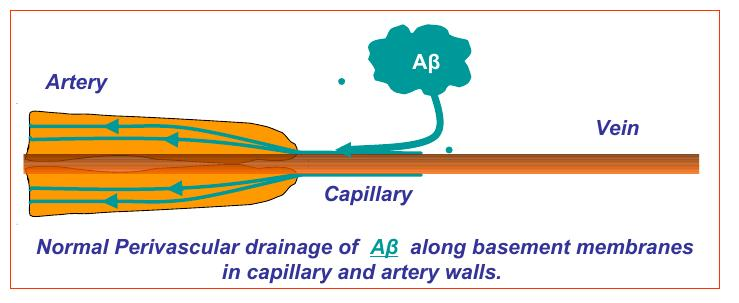
\includegraphics[scale=0.6]{drainage.jpg}
                \caption{Perivascular drainage of A$\beta$ along basement membranes.}\label{fig:1}
\end{figure}

With ageing and a certain genetic disposition soluble A$\beta$ is not eliminated from the brain, instead it is deposited in the walls of blood vessels as \emph{Cerebral Amyloid Angiopathy} (CAA) \cite{Rox,;wellerperi}. CAA may cause a blockage in the ISF drainage pathways resulting in an alteration of the composition of ISF in the brain parenchyma. This change in biochemical composition of the ISF leads to nerve cell death and Alzheimer's Disease. \cite{Rox}.   

\begin{figure}[h]

              \centering
               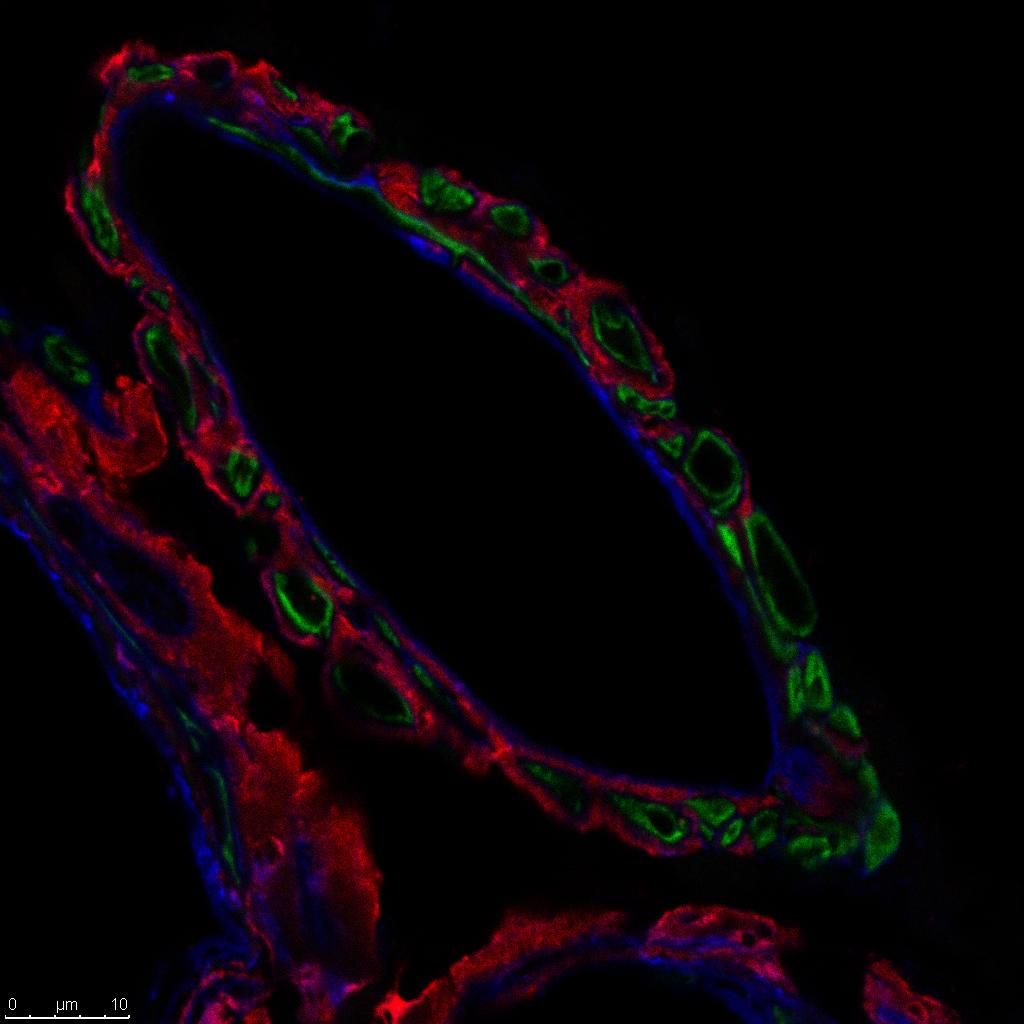
\includegraphics[scale=0.15]{abeta.jpg}
                \caption{CAA in a cross-section of a leptomeningeal artery: the deposition of A$\beta$ is shown in red.  The walls of cerebral capillaries consist of one fused layer of basement membrane which is approximately 150 nm in thickness.}\label{figy:2}
\end{figure}

Susceptibility to CAA varies throughout the brain and vascular vessels.  In particular  
CAA  is most prominent in the occipital, temporal and frontal lobes and least prominent in the parietal lobe and the cerebellum %The leptomeningeal and cortical arteries are particularly prone to CAA whereas CAA is very rare in capillaries 
\cite{Preston}. We suspect that one reason for the differing unacceptability of CAA is the differing symmetry of the cerebral arterial tree.  High levels of symmetry have been shown to be advantageous in other networks.  For example Song \emph{et al.} found that a fractal biochemical annotation  network (a graph with a high level of symmetry) is more robust than a less symmetric graph \cite{Song}.  In order to test the hypothesis that symmetry effects susceptibility to CAA we design and implement a graph theoretic algorithm that models CAA.%and therefore need to make some relevant definitions from graph theory.  


\section{Background}

In Section \ref{sec:meth} we will describe an algorithm that models CAA.  This algorithm is constituted of two parts; a model of the anatomical structure of the perivascular drainage system and a process that replicates the accumulation of A$\beta$.  We will describe this model in the language of graph theory; reformulating CAA as a graph process.      

\subsection{Graphs and Trees}
Graph theory has a rich mathematical history dating back to Leonard Euler although more recently graph theory, under the guise of the much ballyhooed \emph{Science of Networks}, has been applied to model diverse phenomena such as social networks, the world wide web, and the Internet \cite{barabasi,bigg}.

Graphs are mathematical structures comprising of points called ``vertices'' and lines between them called ``edges''.  Graphs are drawn with a dot or circle for each vertex and a line between each dot if there is an edge between them.  See Figure \ref{fig:1} for an example of a graph.     

A (undirected, unweighted) graph is a pair $G = (V(G),E(G))$ such that $V(G)$ and $E(G)$ are the vertices and edges of $G$ respectively. Every edge $e \in E(G)$ begins and ends at vertices $ v,w \in V(G)$. If an edge begins and ends at the same vertex we call that edge a \emph{loop}.  We say that two vertices are \emph{adjacent} if they are connected via an edge.

It is possible to encode more information in a graph by giving each edge a number or \emph{weight}.  For example, a graph representing a road network with vertices as junctions and edges as roads could usefully be weighted by the capacities of each road.  We depict a weighted graph as a by writing the weight of each edge next to that edge.  

%\begin{ex}
 \definecolor{cff0000}{RGB}{255,0,0}
 \definecolor{c770d0c}{RGB}{119,13,12}
\definecolor{c30a3f9}{RGB}{48,163,249}
\begin{figure}[H]
\centering
\begin{tikzpicture}[y=0.80pt,x=0.80pt,yscale=-1, inner sep=0pt, outer sep=0pt, scale = 0.3]
  \path[cm={{1.64548,0.08392,-0.09385,1.47135,(-193.31641,-165.94688)}},draw=black,fill=c770d0c,fill
    opacity=0.000] (553.0000,211.3622)arc(0.000:180.000:72.500000 and
    76.000)arc(-180.000:0.000:72.500000 and 76.000) -- cycle;
  \path[shift={(259.0,392.0)},fill=c30a3f9]
    (285.7143,239.5050)arc(0.000:180.000:80.000000 and
    78.571)arc(-180.000:0.000:80.000000 and 78.571) -- cycle;
  \path[shift={(-116.0,394.0)},fill=c30a3f9]
    (285.7143,239.5050)arc(0.000:180.000:80.000000 and
    78.571)arc(-180.000:0.000:80.000000 and 78.571) -- cycle;
  \path[shift={(249.0,42.0)},fill=c30a3f9]
    (285.7143,239.5050)arc(0.000:180.000:80.000000 and
    78.571)arc(-180.000:0.000:80.000000 and 78.571) -- cycle;
  \path[fill=black,line join=miter,line cap=butt,line width=0.800pt] (0,0)
    node[above right] (flowRoot4017) {};
  \path[xscale=1.004,yscale=0.996,fill=black] (421.98358,660.8728) node[above
    right] (text4025) {V3};
  \path[xscale=0.896,yscale=1.116,fill=black] (63.534481,597.77637) node[above
    right] (text4033) {V2};
  \path[xscale=0.817,yscale=1.224,fill=black] (514.15002,252.65466) node[above
    right] (text4037) {V1};
  \path[draw=black,line join=miter,line cap=butt,line width=0.800pt]
    (168.0000,641.3622) -- (382.0000,638.3622);
  \path[draw=black,line join=miter,line cap=butt,line width=0.800pt]
    (463.0000,550.3622) -- (461.0000,359.3622);
  \path[draw=black,line join=miter,line cap=butt,line width=0.800pt]
    (382.0000,309.3622) -- (137.0000,569.3622);

\end{tikzpicture}
\caption{A graph with 3 vertices, 4 edges and 1 loop.  The path 1-2-3 is a cycle}\label{fig:1}
\end{figure}
%\end{ex}

It is said that it is not what you know but who you know that counts and this is especially true in the case of graphs. Each vertex ``knows'' the vertices connected by an edge to itself and each edge incident to a vertex links that vertex to others in the network. In addition, ``How many you know'' is a significant quantum of information given by a graph as the number of edges incident to a vertex.  One might ask what happens if we traverse a network begining at a vertex and traversing consecutive edges, later arriving at another vertex. In particular we might ask, can we traverse the network and return to the same vertex we started at without traversing an edge more than once. In the example of a road network this is equivalent to asking whether we can drive from one junction to another without driving along a road (in either direction) more than once.         

The degree, $\deg(v)$, of a vertex $v$ is the number of edges incident to $v$.  If $\deg(v) = 1$ then we say that $v$ (and the edge incident to $v$) is a  \emph{leaf}. A path is a sequence of distinct consecutive edges and a cycle is a path beginning and ending at the same vertex that doesn't visit an edge more than once.  A \emph{tree} is  a connected graph (there exists a path between every pair of vertices) which admits no cycles or loops \cite{bela}.  

The appropriate graph to model a phenomenon will have properties such as a restriction on the degree of a particular or all of the vertices.  If the degree of every vertex of a tree is 3 or less then we call that tree a \emph{binary} tree.  For example, the tree depicted in Figure \ref{fig:2} is \emph{not} a binary tree since $\deg(V2) = 4$.

%\begin{ex}
 \definecolor{cff0000}{RGB}{255,0,0}
 \definecolor{c30a3f9}{RGB}{48,163,249}
\definecolor{cff0d0c}{RGB}{255,13,12}

\begin{figure}[H]
\centering




\begin{tikzpicture}[y=0.80pt,x=0.80pt,yscale=-1, inner sep=0pt, outer sep=0pt, scale = 0.3]
  \path[shift={(175.0,149.0)},fill=c30a3f9]
    (285.7143,239.5050)arc(0.000:180.000:80.000000 and
    78.571)arc(-180.000:0.000:80.000000 and 78.571) -- cycle;
  \path[shift={(-111.0,507.0)},fill=c30a3f9]
    (285.7143,239.5050)arc(0.000:180.000:80.000000 and
    78.571)arc(-180.000:0.000:80.000000 and 78.571) -- cycle;
  \path[shift={(174.0,503.0)},fill=c30a3f9]
    (285.7143,239.5050)arc(0.000:180.000:80.000000 and
    78.571)arc(-180.000:0.000:80.000000 and 78.571) -- cycle;
  \path[shift={(435.0,490.0)},fill=c30a3f9]
    (285.7143,239.5050)arc(0.000:180.000:80.000000 and
    78.571)arc(-180.000:0.000:80.000000 and 78.571) -- cycle;
  \path[shift={(177.0,-157.0)},fill=cff0d0c]
    (285.7143,239.5050)arc(0.000:180.000:80.000000 and
    78.571)arc(-180.000:0.000:80.000000 and 78.571) -- cycle;
  \path[draw=black,line join=miter,line cap=butt,line width=0.800pt]
    (380.0000,163.3622) -- (382.0000,318.3622);
  \path[draw=black,line join=miter,line cap=butt,line width=0.800pt]
    (326.0000,450.3622) -- (326.0000,449.3622) -- (138.0000,685.3622);
  \path[draw=black,line join=miter,line cap=butt,line width=0.800pt]
    (382.0000,469.3622) -- (380.0000,663.3622);
  \path[draw=black,line join=miter,line cap=butt,line width=0.800pt]
    (444.0000,441.3622) -- (600.0000,669.3622);
  \path[fill=black,line join=miter,line cap=butt,line width=0.800pt] (0,0)
    node[above right] (flowRoot4017) {};
  \path[fill=black] (72,762.36218) node[above right] (text4025) {V3};
  \path[fill=black] (358,402.36218) node[above right] (text4033) {V2};
  \path[fill=black] (357,93.362183) node[above right] (text4037) {V1};
  \path[fill=black] (358,764.36218) node[above right] (text4041) {V4};
  \path[fill=black] (615,746.36218) node[above right] (text4045) {V5};

\end{tikzpicture}
\caption{Tree, $T$ with edges $\{(V1V2)(V2V3)(V2V4)(V2V5)\}$.  We may permute edges $\{ (V2V3)(V2V4)(V2V5)\}$ whilst preserving adjacent vertices in 6 possible ways so $\lvert \Sym(T)\rvert = 6$. By assigning $V1$ to be the root of $T$ notice that $\lv(V1) = 0, \lv(V2) = 1, \lv(V3) = \lv(V4) = \lv(V5) = 2.$.  The vertices marked in blue represent an induced subtree of $T$, rooted at V2. 
}\label{fig:2}  
\end{figure}
%\end{ex}

One might describe an object as symmetric if it can be rotated or reflected in such a way that the object looks ``the same'' after the rotation or reflection.  Similarly a graph can be described as symmetric if that graph looks the same after we have shifted edge and vertices.    

\begin{rem}
One can formally calculate the symmetry of a mathematical object such as a graph or cube by identifying that object's \emph{group of symmetries}.  For example the group of (orientation preserving) symmetries of the cube consist of all possible rotations of the cube i.e. how can one pick a cube up and rotate it in such a way that when we put it down it looks identical to the original cube.  Similarly, for a tree $T$ the group of symmetries, $\Sym(T)$, consists of all permutations of vertices/edges that preserve vertex adjacency. The number of possible legal permutations is written as $\lvert\Sym(T)\rvert$ and we say that a tree with a larger number of legal permutations is more \emph{symmetric} than a tree with a smaller symmetry group.  
\end{rem}

The vascular system comprises of a hierarchy of vessels: blood flows from arteries to arterioles to capillaries.  To reflect this hierarchy our model will incorporate a \emph{rooted} tree: a tree in which one vertex has been assigned the role of \emph{root}.  The assigned root vertex in our model will correspond to the point where A$\beta$ drains out of the cerebral vasculature and into the lymphatic system. The \emph{level} of each vertex $v \in V(G)$ is the length of the shortest path from $v$ to the root; we write this as $\lv(v)$.


Recall from Section \ref{sec:intro} the hypothesis that there exists correlation between a high degree of symmetry and network robustness. To gain some intuition into this hypothesis consider the following (extreme) example.  Let $T_1$ be the tree on 15 vertices depicted on the left and $T_{2}$ be the line of 15 vertices depicted on the right of Figure \ref{fig:silly} [below].

These trees have the same number of vertices and edges but hugely different symmetry groups.  Imagine that fluid flows on $T_1$ and $T_2$ and that fluid always flows towards vertex the root vertex (labelled 1).  If we remove an edge from either tree then all the edges flowing into that edge become redundant.  Tree $T_2$ is significantly more vulnerable to attack because if we remove an edge from $T_2$ all the edges to the right of the removed edge are rendered useless.  Whereas, if we remove an edge from $T_1$ we only remove the edges lower than the removed edge.

Since $|\Sym(T_{1})| = 128$ and that $|\Sym(T_{2})|$ = 2, $T_{1}$ is more symmetric than $T_{2}$.  

\begin{figure}[H]
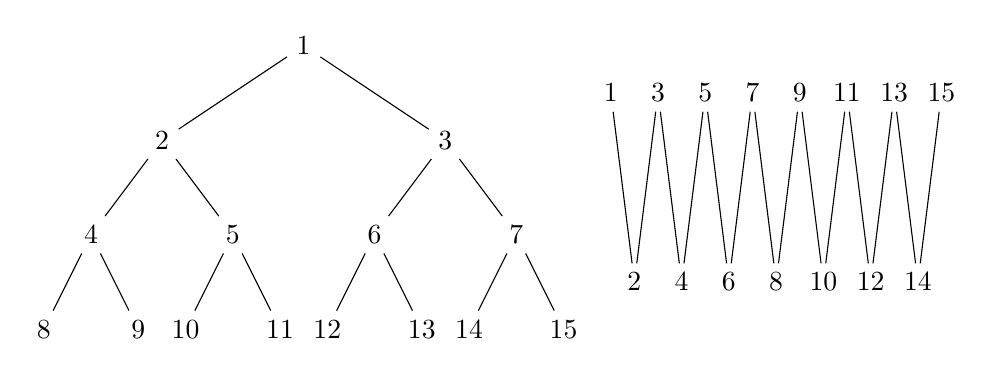
\begin{tikzpicture}[scale = 0.6]
  [scale=0.9,auto=left,every node/.style={circle,fill=blue!20}]
  \node (n1) at (5.5,7) {1};
  \node (n2) at (2.5,5)  {2};
  \node (n3) at (8.5,5)  {3};
  \node (n4) at (1,3) {4};
  \node (n5) at (4,3)  {5};
  \node (n6) at (7,3)  {6};
\node (n7) at (10,3)  {7};
\node (n8) at (0,1)  {8};
\node (n9) at (2,1)  {9};
\node (n10) at (3,1)  {10};
\node (n11) at (5,1)  {11};
\node (n12) at (6,1)  {12};
\node (n13) at (8,1)  {13};
\node (n14) at (9,1)  {14};
\node (n15) at (11,1)  {15};

\node (n16) at (12,6)  {1};
\node (n17) at (12.5,2)  {2};
\node (n18) at (13,6)  {3};
\node (n19) at (13.5,2)  {4};
\node(n20) at (14,6)  {5};
\node (n21) at (14.5,2)  {6};
\node (n22) at (15,6)  {7};
\node (n23) at (15.5,2)  {8};
\node (n24) at (16,6)  {9};
\node (n25) at (16.5,2)  {10};
\node (n26) at (17,6)  {11};
\node (n27) at (17.5,2)  {12};
\node(n28) at (18,6)  {13};
\node (n29) at (18.5,2)  {14};
\node (n30) at (19,6)  {15};

  \foreach \from/\to in {n1/n2,n1/n3,n2/n4,n2/n5,n3/n6,n3/n7,n4/n8,n4/n9,n5/n10,n5/n11,n6/n12,n6/n13,n7/n14,n7/n15,n16/n17,n17/n18,n18/n19,n19/n20,n20/n21,n21/n22,n22/n23,n23/n24,n24/n25,n25/n26,n26/n27,n27/n28,n28/n29,n29/n30}
    \draw (\from) -- (\to);

\end{tikzpicture}
\caption{$T_{1}$ and $T_{2}$}\label{fig:silly}
\end{figure}
If we remove an edge at random from $T_{1}$ and also remove the  induced subtree adjacent to that edge the expected number of edges removed is:
\begin{equation}
1\frac{8}{14} + 3\frac{4}{14} + 7\frac{2}{14} = \frac{12}{7} 
\end{equation} 
If we remove an edge at random from $T_{2}$ and also remove the  induced subtree adjacent to that edge the expected number of edges removed is:
\begin{equation}
\frac{1}{14}\sum_{k=1}^{14}k = \frac{15}{2} > \frac{12}{7}
\end{equation}


\subsection{Anatomical data}\label{sec:ana}

In order to build an effective model of CAA we will incorporate relevant anatomical data such as arterial length, branching and the radius of vessels \footnote{  There is  a great deal of disagreement and ambiguity in the literature pertaining to arterial vessel segments and branching points \cite{Zamir}.  We will use the definitions given by Cassot \emph{et al.} \cite{Cassot}} in our model.
Cassot \emph{et al.} conducted a detailed analysis of the cerebral vasculature which has formed the basis of numerous numerical analyses \cite{grinberg,francis}. Cassot \emph{et al.} found that 98\% of branching in the cerebral cortex is bifurcation and there are approximately  300 branching points \cite{Cassot}. 


At an arterial bifurcation point with parent vessel $p$ and daughter vessels $d_{1}$ and $d_2$ Murray's law \cite{Murray} states that:

\[r_{p}^{3} = r_{d_{1}}^{3} + r_{d_{2}}^{3}\]
where $r_{p}$ is the radius of $p$ and $r_{d_{1}},r_{d_{2}}$ are the radii of $d_{1}$ and 
$d_{2}$ respectively.
Experimental evidence has shown that Murray's law is a good approximation for 
arterial vessels \cite{Zamir,cohn}.

Murray's law describes the relationship between certain bifurcating  
\emph{cylindrical vessels}, however we will model the cerebral perivascular pathways as \emph{annular prisms}.  Therefore we will adjust Murray's law to describe 
the relationship between parent and child annular prisms. In addition we assume that the width of the perivascular space, $\epsilon$, is the same for any vessel from capillary to
 artery. Since the notion of radius is more 
complicated for an annular prism we reformulate Murray's law in terms of 
cross-sectional area in Lemma \ref{lem:murr}.   

%insert diagram here

\begin{lem}[Murray's law adjusted for annular prisms]\label{lem:murr}
Let the parent vessel have radius $r_{p} = r_{p}' + \epsilon$ and the two 
daughter vessels have radii $r_{d_i} = r_{d_i}' + \epsilon$ for $i = 1,2$.
 \[A_p = \pi\left(\epsilon^{2} + 2\epsilon \left(\left( \frac{A_{d_{1}} + \pi\epsilon^{2}}{2\epsilon\pi} \right)^{3} + \left( \frac{A_{d_{2}} + \pi\epsilon^{2}}{2\epsilon\pi} \right)^{3}\right)^{\frac{1}{3}}\right)\]
where $A_p$ is the cross-sectional area of the parent vessel and $A_{d_{1}}$ and $A_{d_{2}}$ are the cross-sectional areas of the two daughter vessels at a bifurcation.
\end{lem}
\begin{proof}
The relationship between the cross-sectional area, $A_{X}$ of any vessel and the radius, $r_{X}$ 
of that vessel is given by the formulae:
\begin{align*}
 A_{X} &= \pi((r_{X}' + \epsilon)^{2} - r_{X}'^{2})\\
 &= \pi(\epsilon^{2} + 2\epsilon r_{X}')\\
 r_{X}' &= \frac{A_{X} - \pi\epsilon^{2}}{2\epsilon\pi}\\
 r_{X} &=  \frac{A_{X} - \pi\epsilon^{2}}{2\epsilon\pi} + \epsilon \\
 &= \frac{A_{X} + \pi\epsilon^{2}}{2\epsilon\pi}
\end{align*}

By combining the above equations we find that the cross-sectional area of the parent
 vessel, $A_{p}$, is given by:

\begin{align*}
A_{p} &= \pi(\epsilon^{2} + 2\epsilon r_{p}) \\
&= \pi\left(\epsilon^{2} + 2\epsilon (r_{d_{1}}^{3} + r_{d_{2}}^{3})^{\frac{1}{3}}\right)\\
&= \pi\left(\epsilon^{2} + 2\epsilon \left(\left( \frac{A_{d_{1}} + \pi\epsilon^{2}}{2\epsilon\pi} \right)^{3} + \left( \frac{A_{d_{2}} + \pi\epsilon^{2}}{2\epsilon\pi} \right)^{3}\right)^{\frac{1}{3}}\right)
\end{align*}
\end{proof}

\section{Method}\label{sec:meth}

In this section we will describe the algorithm we designed to replicate CAA \footnote{This algorithm was implemented using the numerical modelling program \emph{matlab} \cite{matlab}}.  This algorithm has three constituent parts:
\begin{itemize}
\item[(i)] Generate 50 random rooted trees; $\mathcal{T} = \{ T_1,T_2,\dots,T_{50}\}$.
\item[(ii)]Calculate the order of the symmetry group of each tree using the graph isomorphism program \emph{nauty} \cite{nauty}.
\item[(iii)] Replicate CAA by removing edges $e \in E(T_i)$. 
\end{itemize} 

Each tree encodes the anatomical information discussed in Section \ref{sec:ana}. Graphical characteristics of each tree such as the degree of each vertex were determined by the anatomical survey of cerebral vascular trees carried out by Cassot \emph{et al.} \cite{Cassot}.  However, since we are modelling perivascular drainage rather than blood flow each branch was assigned a number representing the total volume of the basement membrane enveloping the relevant arterial tree.   

Each rooted binary tree was generated with $300$ vertices and every edge $e \in E(T_i)$ was associated with an annular prism and assigned a volume $\vol(e)$.   Leaf  edges were defined to have volume 1 and subsequent edges were given a volume consistent with Murray's law for annular prisms (see Lemma \ref{lem:murr}).  

The fundamental assumption we made when we replicated CAA was that it is more likely for an edge to succumb to CAA if the concentration of A$\beta$ in that edge is higher.  Since the production of A$\beta$ is approximately constant throughout a human lifetime \cite{wellerperi} we assumed that the rate of removal of $A\beta$ into the lymphatic system (the root vertex in our model) was constant. This implies that when a vascular unit becomes blocked via CAA the concentration of A$\beta$ in the intact perivascular pathways increases forming a devastating negative feedback loop.  Our model incorporated these assumptions by calculating the concentration of A$\beta$ in terms of the functioning part of the weighted, rooted , binary tree. 

A blockage in the perivascular system was modelled by the removal of an edge from $T_i$.  Such a blockage in the basement membrane results in a failure of drainage from all vessels that feed that edge. Therefore, if the edge joining vertices $v,w \in V(T)$ was removed and (without loss of generality) $\lv(v) < \lv(w)$ then we also removed the induced subtree rooted at $w$ from $T_i$.     
    

The \emph{initial} volume of each tree $T_i$ was defined to be 
\[\Vol(T_i) =  \sum_{e \in E(T_i)} \vol(e)\]
 
The process of edge removal proceeds as follows:  at time $t=0$ we set $T_{i}(0) = T_{i}$ (our randomly generated rooted binary tree).  At subsequent times  $t = 1,2,\dots$ we associated a probability $0<P_{t}\leq 1$, that edge $e$ was to be removed at time $t$, with every edge $e \in E(T(t))$. If edge $e$ was removed then the induced subtree rooted at the endpoint of $e$ greatest distance from the root of $T_i$ was also removed to form $T_i(t)$.   

The volume of $T_i$ at time $t$ was defined to be $\Vol_{t}(T_i) = \sum_{e \in E(T_i(t))} \vol(e)$.  We then defined concentration: 
\[C(t) = \frac{\Vol(T_i)}{\Vol_{t}(T_i)}.\]
We can now define %$P = p.C(t)$ where if $pC(t)<1$ and $P = 1$ if $p(C(t)) \GE 1$ for some $0<p<1$.     

\[P_t = \begin{cases} p.C(t) &\mbox{if } p.C(t) <1 \\
1 & \mbox{otherwise }  \end{cases} \text{       where   } 0<p<1 \]

Finally, we recorded the time, $\tau_{i}$, taken to remove half of the edges from each tree $T_{i}$ (henceforth we will refer to $\tau_i$ as the \emph{half-life}). 
 
\section{Results}  

For each tree $T_i$ we calculated the order of the symmetry group $\lvert\Sym(T_i)\rvert$ and the minimum time, $\tau_i$, taken for at least half of the edges $e \in E(T_i)$  to be removed from $T_i$.  We further calculated the median order of symmetry group, $\phi = $, and partitioned $\mathcal{T}$ into two subsets as follows: 

\[\mathcal{T}_{1} = \{T_i \in \mathcal{T} : \lvert\Sym(T_i)\rvert < \phi\} \text{      and      }\mathcal{T}_{2} = \{T_i \in \mathcal{T} : \lvert\Sym(T_i)\rvert \geq \phi\} \]
 
We also calculated the mean values, $\mu_j$ ($j = 1,2$) of $\tau_i$ for trees in $\mathcal{T}_j$ for $j = 1,2$:
\[\mu_j = \frac{\sum_{T_i \in \mathcal{T}_j}}{|\mathcal{T}_j|}\]

Figure \ref{t12} shows the $\mu_j$ corresponding to the $\mathcal{T}_j$

\begin{figure}[H]

              \centering
              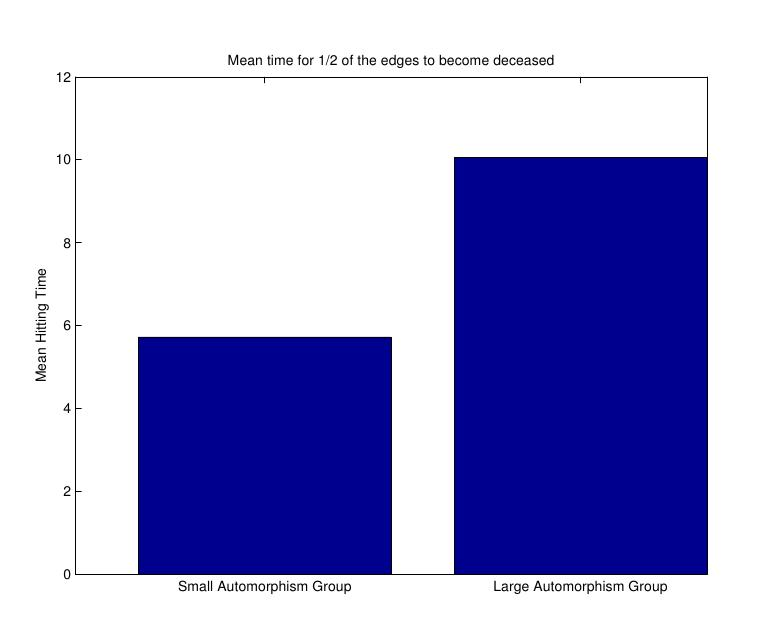
\includegraphics[scale=0.5]{half.jpeg}
                \caption{Mean time for $\frac{1}{2}$ edges to be removed for high and low values of $|\Sym(T_i)|$}\label{t12}
\end{figure}

It is clear that in general the trees with a larger symmetry group had a greater half-life.

\section{Discussion}

In order to place our results back into a medical context recall that the edges and vertices of each tree $T_i$ correspond to arterial vessels and branching points respectively.  The half-life, $\tau_i$ associated with each tree describes the rate at which drainage pathways become obstructed i.e. the rapidity of the onset of CAA.  

In order to build an effective model of CAA it was necessary to make several simplifying assumptions.  We defined the probability that an edge was removed in terms of the concentration of A$\beta$ but the distribution of deposition of A$\beta$ in a real arterial vessel is complex and not yet fully understood %\cite{yow}.
Further, our model of CAA was discrete, i.e. an edge either allowed free flow of ISF or was blocked but in reality CAA is a gradual process.  We would recommend the inclusion of variable edge flow to build a more sophisticated model of CAA. 

Ambrose has shown that the brain undergoes angiogenisis which could be reflected by including a new random parameter which governs the introduction of edges in our algorithm \cite{ambrose}.   Modelling basement membranes as annular prisms does not take into account the tortuous routes of perivascular drainage therefore one might also include a tortuosity parameter in a more refined model.  Finally, we could model arteriosclerosis (suspected to be a major contributing factor to CAA \cite{wellerperi})  by 
introducing a monotonically decreasing radial function. 

Our results suggest that a more symmetric cerebral arterial tree could indicate a higher degree of robustness to CAA, however we stress that ours is a very rudimentary model.  Further evidence of this correlation could be found by experiment examining the relationship between highly symmetric areas of the brain and the extent to which those areas are affected by CAA. 

\section{Conclusion and Clinical Implications}

We have demonstrated that it is likely that there is correlation between symmetry of the cerebral vascularture and lower risk of proliferation of CAA.  

\bibliographystyle{h-physrev3.bst}


\bibliography{./medicine}{}

\end{document}
